\chapter{Introduction}
\label{chap:introduction}

Many established speech enhancement benchmarks and baselines are built around conventional 16 kHz wideband settings. In this setting, the upper-band spectral components contained in 48 kHz full-band speech are outside the model input. Direct 48 kHz full-band speech enhancement therefore presents a different operating condition: the model receives a noisy full-band signal, and the upper-band spectrum is available as noisy evidence to be enhanced. Although full-band enhancement has been explored in prior work, same-protocol references for direct 48 kHz full-band SE remain less established than conventional wideband evaluation.

Speech bandwidth extension and speech super-resolution target a different information condition. These tasks aim to reconstruct missing or degraded high-frequency content from band-limited inputs~\cite{liu2022voicefixer,andreev2022hifiplusplus}, whereas 48 kHz full-band SE starts from a noisy full-band observation. Therefore, the key issue is not to synthesize the upper band after wideband enhancement, but to suppress noise over the full observed spectrum while preserving useful spectral evidence. This distinction motivates a direct full-band enhancement approach in which the high-frequency region is treated as part of the noisy observation rather than as a missing component to be generated afterward.

Practical full-band systems such as PercepNet and DeepFilterNet2 have shown that full-band enhancement can be made feasible under strict computational constraints~\cite{valin2020percepnet,schroter2022deepfilternet2}. PercepNet uses perceptually motivated critical-band features and comb filtering, while DeepFilterNet2 combines ERB-domain enhancement with deep filtering. Such perceptual-band front ends trade bin-level spectral resolution for efficiency, which motivates a complementary TF-domain design that uses a learned frequency representation and estimates the enhanced spectrum through complex filtering over the original noisy STFT.

Directly applying heavy TF modeling to all full-band frequency tokens can be computationally costly, especially as the number of STFT bins increases with sampling rate. Since harmonic and formant-related speech-structure evidence is concentrated mainly in lower frequencies while upper-frequency bins remain observed in the noisy input, a natural design is to concentrate heavier encoding on low-band structure and carry the high band as decoder-side observed-query evidence.

In this work, we propose TF-Rehancer, a refinement-oriented time-frequency architecture for direct full-band speech enhancement. The core idea is low-band-guided full-band refinement. TF-Rehancer concentrates heavier encoding on low-band speech structure, preserves observed upper-band evidence in the decoder path, and estimates the enhanced spectrum through complex filtering over the original noisy STFT. This design allows the model to exploit cross-band speech structure while keeping the final estimation tied to the observed noisy signal.

From the attention perspective, the low-band encoder output provides key/value context for the high-band portion of the decoder representation. Cross-attention updates the observed high-band decoder tokens, after which full-sequence decoder modules model the joint low- and high-band representation. Thus, TF-Rehancer does not generate high-band speech from low-band information alone; it uses low-band context to condition the update of observed high-band features.

\begin{figure}[t]
    \centering
    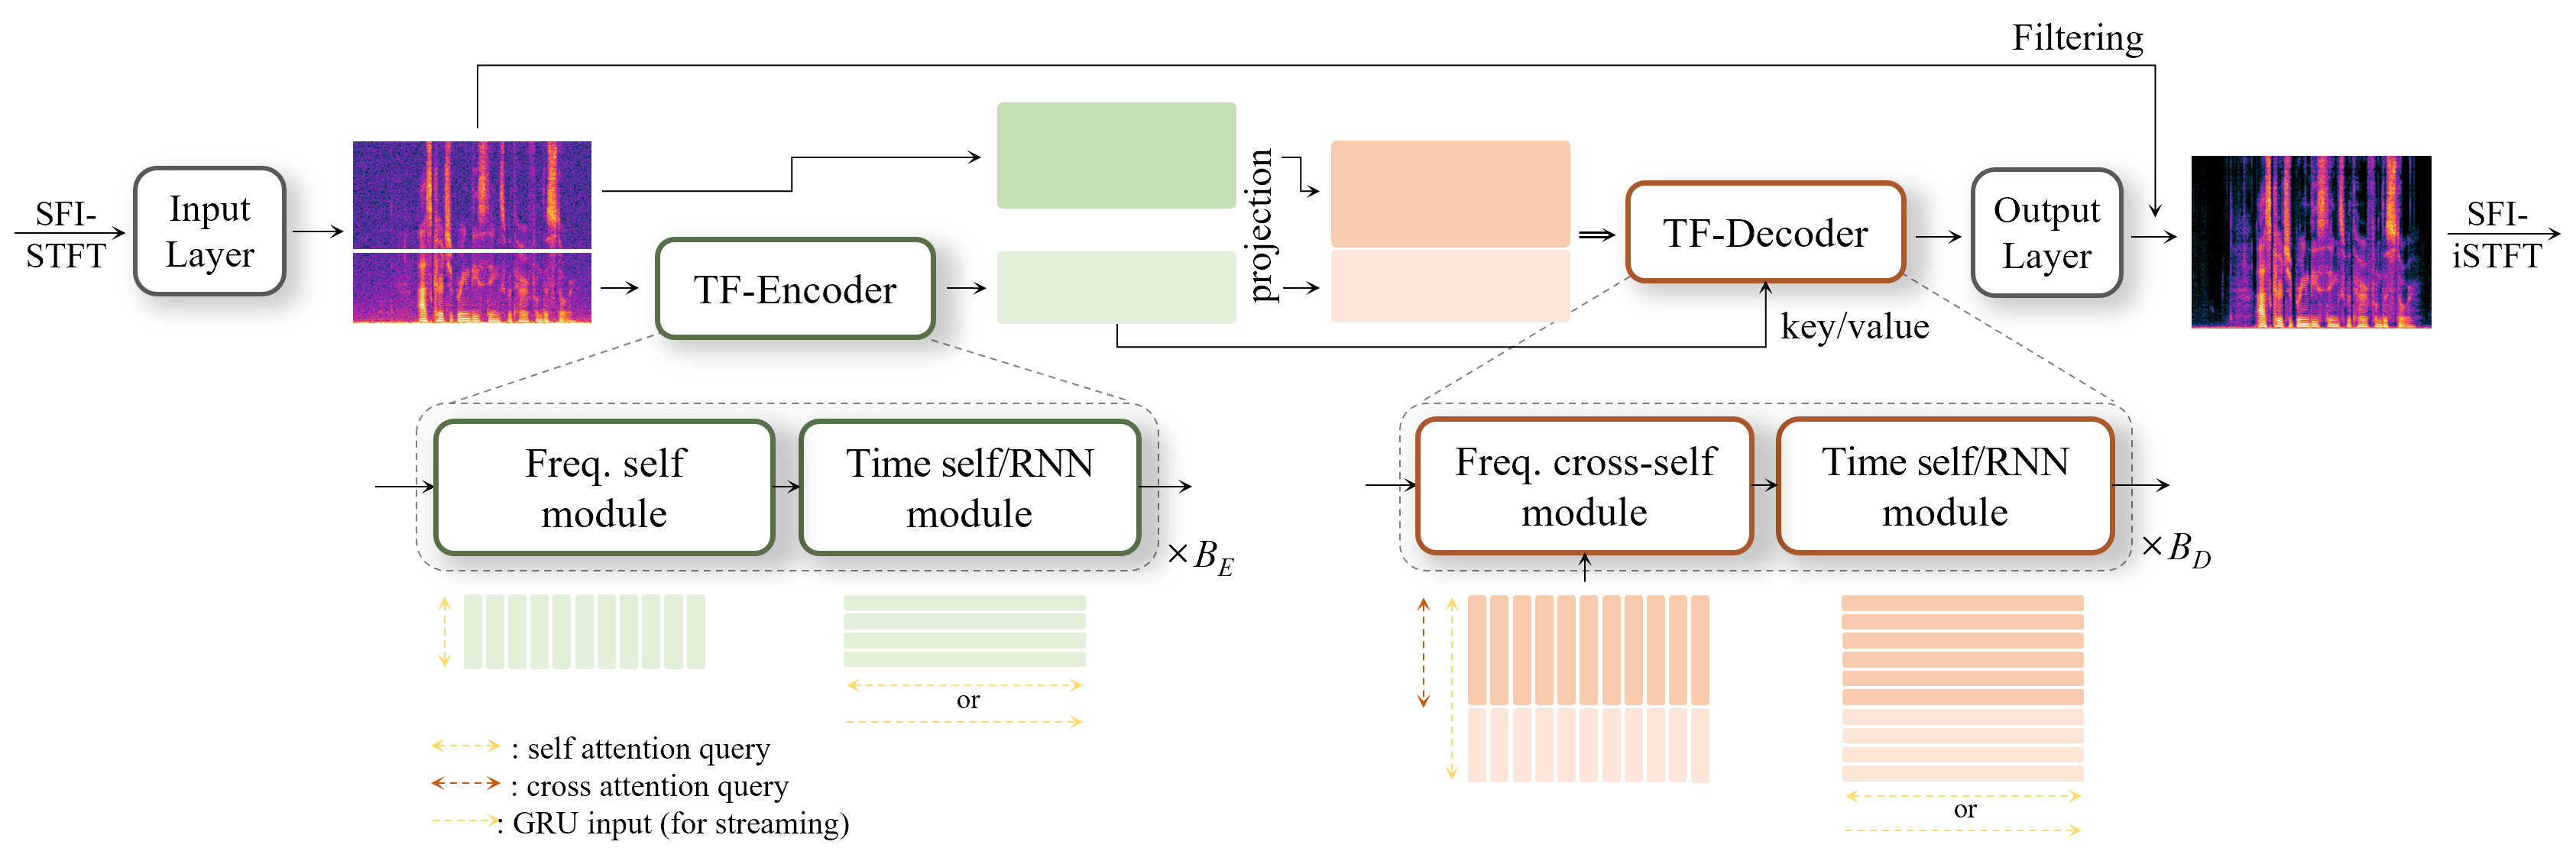
\includegraphics[width=0.92\textwidth]{figures/Overall_Model_Flow.png}
    \caption[Conceptual overview of TF-Rehancer]{Conceptual overview of TF-Rehancer. The low-band encoder output provides key/value context for updating the observed high-band decoder tokens. The updated representation is then processed by full-sequence decoder modules and used to estimate local complex filters over the original noisy STFT.}
    \label{fig:intro_tf_rehancer_overview}
\end{figure}

We evaluate TF-Rehancer in three settings. The first is 48 kHz full-band results on the VoiceBank+\allowbreak DEMAND 48 kHz test set against published full-band references. The second is a 16 kHz VoiceBank+\allowbreak DEMAND quality-efficiency comparison. The third is controlled 48 kHz ablation analysis of the proposed architecture.

The contributions of this work are summarized as follows.
\begin{enumerate}
    \item We formulate 48 kHz full-band SE as observation-preserving refinement, where upper-band components are treated as noisy spectral evidence rather than missing content to be generated after wideband processing.
    \item We propose TF-Rehancer, a TF-domain architecture for low-band-guided full-band refinement. It updates observed high-band decoder tokens using low-band encoder context, models the resulting full embedded sequence, and estimates the enhanced spectrum through complex filtering over the noisy STFT.
    \item We evaluate TF-Rehancer through 48 kHz full-band results against published full-band references, a 16 kHz quality-efficiency comparison, and controlled 48 kHz ablations of complex filtering, decoder cross-attention, and the low-band cutoff.
\end{enumerate}

The remainder of this thesis is organized as follows. Chapter~\ref{chap:related_work} reviews related work in wideband enhancement, bandwidth extension, and practical full-band enhancement. Chapter~\ref{chap:proposed_method} describes the TF-Rehancer architecture and training objective. Chapter~\ref{chap:experiments} presents the experimental setup, benchmark results, and ablation analysis. Chapter~\ref{chap:conclusion} summarizes the thesis and discusses limitations and future work.
